\section{Protocol Implementation}

\subsection{Carry Slot Contract}

Carry Protocol manages game advertisements through slots. The protocol itself serves as the smart contract which manages the lifecycle of advertisement contents and slots.
\begin{figure}[!htb]
    \centering
    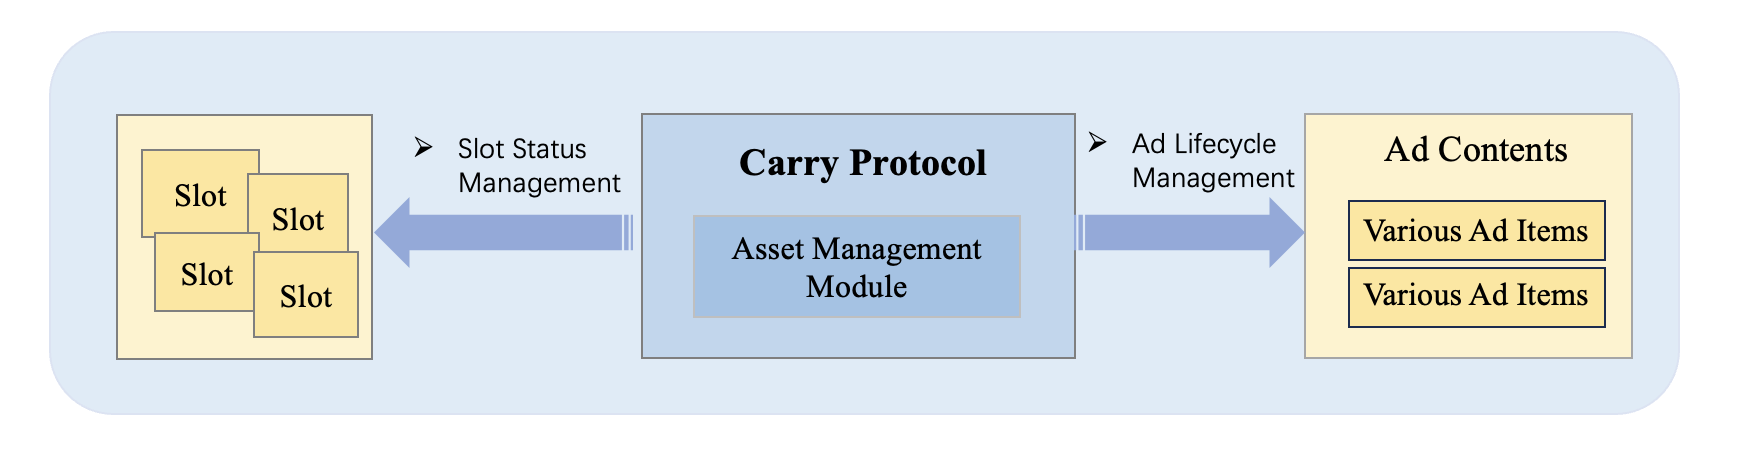
\includegraphics[width=0.9\textwidth]{slotexplain.png}
    \caption{Slot is the basic instrument for Carry Protocol to manage advertisement.}
    \label{fig:slotexplain}
\end{figure}

\subsubsection{Slot Creation}

When a new ad campaign is about to start in a web3 game, the first step is setting up a special ad spot, known as a "slot." This slot is made into a unique digital item, like a one-of-a-kind collectible, which means it's owned and can be traded. Game makers weave these slots into their games, and then either they or the players can activate them, turning them into owned digital assets. It's similar to creating a brand-new collectible item that's ready to be paired with an ad.

\subsubsection{Slot Release}

A slot, once used, may need to be released or made available for future advertisements. This involves the termination or expiration of its current content, making the slot a blank canvas once more. While this could technically be a part of the slot contract, the process's simplicity might not necessitate a full-fledged contract on its own. Instead, it could be an operation under the broader slot management system.


\subsubsection{Slot Content Change}

Over time, advertisements or the content within a slot might need updating or altering. This could be due to changing marketing strategies, game narratives, or even player preferences. The Carry Slot Contract allows for dynamic content modifications, ensuring that the slot remains relevant and engaging. However, it is challenging to alter the embedded contents since slots are mined as valuable assets which are recorded onto blockchain, which exhibits extreme immutability. Therefore, we need to trade off between modifiability and immutability in Carry \cite{ye2023survey}. To this end, we introduce Chameleon Hash algorithm to achieve a redactable transaction property for Carry. The structure is illustrated in Figure\ref{fig:chameleon}~\cite{wu2021quantum}.

\begin{figure*}[!htb]
    \centering
    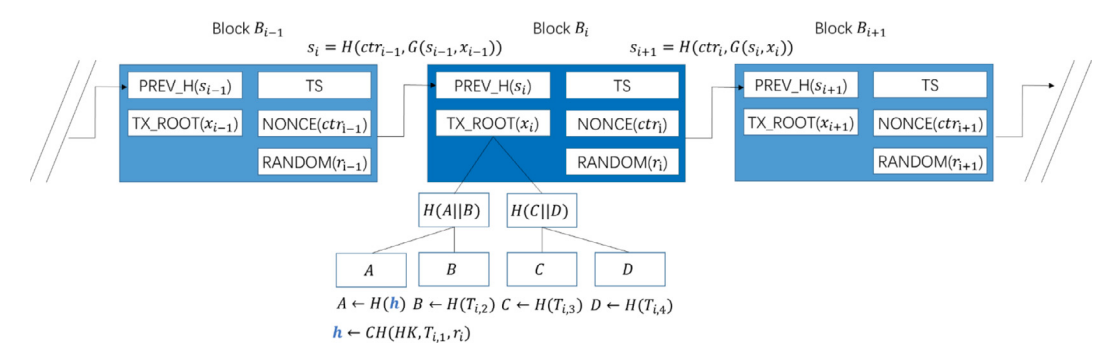
\includegraphics[width=\textwidth]{chameleon hash.png}
    \caption{Chameleon Hash-based Alterable Slot Contents Solution.}
    \label{fig:chameleon}
\end{figure*}

\begin{enumerate}[label=(\arabic*)]
    \item \textbf{Bilinear Pairing.} Let $\mathbb{GF}(p)$ denote a finite field, where $p$ is a large prime number. We consider an elliptic curve $E_p(a,b)$ over $\mathbb{GF}(p)$, which can be defined as the set of ordered pairs $(x,y) \in \mathbb{GF}(p) \times \mathbb{GF}(p)$ that fulfill the condition $y^2 \equiv x^3 + ax + b \;(\text{mod}\; p)$, given that $a, b \in \mathbb{GF}(p)$ and $4a^3 + 27b^2 \not\equiv 0\; (\text{mod}\; p)$. This leads to the construction of an additive cyclic group, denoted $\mathbb{G}_1$, and a multiplicative cyclic group, $\mathbb{G}_2$, both of which have the prime order $p$. These groups are constituted of all points residing on the elliptic curve, complemented by the point at infinity. A random generator of $\mathbb{G}_1$ is designated as $P$. We define a bilinear map $e: \mathbb{G}_1 \times \mathbb{G}_1 \rightarrow \mathbb{G}_2$ (known as a type-1 pairing) that adheres to the following three properties \cite{bagga2023bilinear}:
\begin{itemize}
    \item \textbf{Bilinearity:} For any $X, Y \in \mathbb{G}_1$ and any $a, b \in \mathbb{Z}_p^\ast$, it holds that $e(aX, bY) = e(X, Y)^{ab}$.

\item \textbf{Non-degeneracy:} If we designate $1_{\mathbb{G}_2}$ as the identity element of $\mathbb{G}_2$, it should be ensured that $e(X, Y) \neq 1_{\mathbb{G}_2}$ for any $X, Y \in \mathbb{G}_1$.

\item \textbf{Computability:} For any $X, Y \in \mathbb{G}_1$, the value $e(X, Y)$ can be efficiently computed.
\end{itemize}
    \item \textbf{Complexity Assumptions.} Two fundamental problems play a crucial role in ensuring the robustness of our protocol. These problems \cite{jalaja2023new,mahdavi2023new}, known as the Discrete Logarithm Problem (DLP) and the Computational Diffie-Hellman Problem (CDHP), are outlined below: Given $(g,y)$, where $y\in \mathbb{G}$, the advantage for any probabilistic polynomial time (PPT) adversary to find an integer $x\in \mathbb{Z}_q^\ast$ such that $g^x=y$ is negligible. Given $(g,g^x,g^y)$, where $x,y\in \mathbb{Z}_q^\ast$, the advantage for any PPT adversary to find an element $g^{xy}\in \mathbb{G}$ is negligible.
    \item \textbf{Initialization.} The initialization phase is mainly to initialize the parameters of the elliptic curve cryptosystem and construct the public and private key information.
    \begin{itemize}
        \item The protocol generates elliptic curves $E$ of order $q$, generator $P$, a cyclic additive group $\mathbb{G}$, and the large integer group $\mathbb{Z}_q^\ast$. 
        \item Then, it generates random number $SK$ from $\mathbb{Z}_q^\ast$ as the private key, then calculates $PK = SK\cdot P$, and constitutes its public and private key information $(PK,SK)$. 
        \item Moreover, it selects a Chameleon Hash function $H:CH(g,h,r,t)$, three one-way secure hash functions that $H_1:\{0,1\}^\ast\rightarrow \mathbb{Z}_q^\ast$, $H_2:\{0,1\}^\ast\times \mathbb{G}\rightarrow \mathbb{Z}_q^\ast$, and $H_3: \mathbb{G} \times \{0,1\}^\ast \times \mathbb{G} \times \{0,1\}^\ast \rightarrow \mathbb{Z}_q^\ast$. 
        \item Finally, Carry protocol publishes $\{E,\mathbb{G},P,q,H,H_1,H_2,H_3,PK\}$ as public parameters in the ecosystem.
     \end{itemize}
    \item \textbf{Construction.} The DLP is leveraged to construct the chameleon hash function. First, the entity who wants to change the contents in the slot generates a random value $SK_u \in \mathbb{Z}_q^\ast$ from the group of integers as his/her private trapdoor key, and the group $\mathbb{G}$ generates a trapdoor to create the public key $g$. The public trapdoor key $h$ is obtained by computing $h=g^{SK_u}$.

    A random value $r$ is generated at time $T_u$, where $r \in \mathbb{Z}_q^\ast$. The value of the Chameleon Hash function $T_u$ is obtained by calculating $H$. The construction and calculation of $H_2$ is given by the following equation:
    \begin{equation}
       H= CH(g,h,r,T_u)=\big(g^{T_u}\big)\cdot h^r=g^{T_u+(SK_u)\cdot r}
    \end{equation}
\end{enumerate}

Since changing the random value $r$ will definitely lead to a change in the chameleon hash function value, the hash value of the current time $T_n$ is calculated by Equation (4) when $T_u$ becomes $T_n$. In order to make the hash function value of time $T_n$ and that of time $T_u$ the same, i.e., Equation (5) holds, a new random value $r'$ can be calculated by Equation (6). So far, the entity can calculate different time according to the corresponding random value, and thus generate the same hash value.

\begin{equation}
    h_n=CH(g,h,r',T_n)=\big(g^{T_n}\big)\cdot h^{r'}=g^{T_n+(SK_u)\cdot r'}
\end{equation}
\begin{equation}
\begin{aligned}
      h_n=H& \Rightarrow CH(g,h,r',T_n)=CH(g,h,r,T_u) \\
      & \Rightarrow g^{T_u+(SK_u)\cdot r}=g^{T_n+(SK_u)\cdot r'} \\
\end{aligned}
\end{equation}

\begin{equation}
    r'=forge(SK_u,r,T_n,T_u)=\frac{T_u-T_n}{SK_u}+r
\end{equation}

Thus, by employing the aforementioned theoretical foundation and algorithmic principles, we can modify the contents of a specific slot.

\subsubsection{Slot Advertisement Placement}

The ultimate purpose of a slot is to showcase advertisements, a process termed 'placement' within the Carry Protocol. It's where the rubber meets the road. Once an advertisement is place into a slot, the slot illuminates, fulfilling its purpose. Placement could involve various parameters like the duration of the advertisement, its visual aesthetics, and interactivity levels, all governed and managed by the Carry Slot Contract.

In essence, the Carry Slot Contract is the backbone of the slot system within the Carry Protocol. It ensures that every slot's lifecycle, from creation to placement, is managed efficiently, transparently, and in harmony with the game's environment and the players' expectations.




\subsection{SDK Implementation for Carry Protocol}

Carry's Modular GameFi Infrastructure Platform is a significant advancement in the game industry, especially with the recent integration of asset trading into games. This platform assists stakeholders in adapting to the rapidly changing game landscape.

At its core, Carry's game infra includes an extensive data management system. This system allows game operators to collect, analyze, and utilize real-time data crucial for the game's health and growth. Operators can access detailed metrics such as user retention, online hours, asset generation, consumption, and transactions. This level of insight is vital for making informed decisions to adjust game strategies, balance game economies, and enhance player engagement. The platform also provides tools for analyzing on-chain data, offering operators a comprehensive view of how in-game assets are distributed and used within the blockchain ecosystem. 
\subsubsection{Overview}
We introduce a brief SDK implementation roadmap for the proposed Carry Protocol.
\begin{itemize}
    \item Setup and Dependencies: Initialize the Carry SDK with dependencies on selected blockchain libraries and cryptographic protocols. Moreover, architect the SDK to include modules for Asset Management, Identity Management, and Security Guarantee, ensuring modularity and ease of integration.
\item Module Development: Develop each module according to Section 3, implementing the formalized processes and integrating with blockchain networks and cryptographic services.
\item API Design: Create a comprehensive set of APIs for game developers, covering all functionalities provided by the SDK, with clear documentation and examples.
\item Integration Tools and Libraries: Provide tools and libraries for seamless integration of the SDK into existing game development workflows, supporting both Web2 and Web3 environments.
\item Security Audits and Testing: Conduct extensive security audits and testing of the SDK, including unit tests, integration tests, and penetration tests to ensure robustness and security.
\item Deployment and Support: Deploy the SDK for public use, providing detailed documentation, developer guides, and technical support for game developers integrating blockchain features into their games.
\end{itemize}

This comprehensive approach ensures the Carry SDK provides a robust infrastructure for integrating blockchain technology into traditional games, enhancing asset management, identity verification, and security across the gaming ecosystem. When it comes to Asset Transactions, Carry provides solutions for NFT Marketplace and auctioning. Recognizing the importance of liquidity in asset trading, it also supports integration with prominent platforms like PancakeSwap and OpenSea, offering aggregation services that facilitate trading across various marketplaces.
\subsubsection{Asset Management SDK}
To deploy Carry SDK, developers use JSON with HTTP to realize documentation files API as below. Specifically. we design nine common APIs for Assets Management SDK in Carry Protocol:
\begin{enumerate}
    \item \textbf{Get FT Assets in Game}
    \begin{itemize}
        \item Description: Searches for a user's fungible token (FT) assets within a game.
\item Implementation: A GET request to /ftToken/getAssets?appId=\{\%d\}\&uid={\%d} with game ID and user ID as parameters. This API call fetches the user's in-game FT assets, detailing each asset's name, balance, and frozen balance.
\item Response Example: Returns a JSON object listing FT assets, including names and balances, to help developers track and manage in-game currency distribution among users.
 \end{itemize}
\item \textbf{FT Deposit}
\begin{itemize}
        \item Description: Notifies the game of an FT asset deposit.
\item Implementation: A POST request to /ftToken/deposit with details including the game ID, a digital signature, and deposit information (game coin name, amount, transaction hash, and user ID). This API records the deposit transactions of FT assets into the game, crucial for updating user balances.
\item Response Example: Provides confirmation of the deposit process, including transaction status, to ensure accurate record-keeping of asset inflow.
\end{itemize}
\item \textbf{FT PreWithdraw}
\begin{itemize}
        \item Description: Handles the pre-withdrawal process for FT assets, freezing the corresponding assets.
\item Implementation: A POST to /ftToken/preWithdraw including game ID, signature, and withdrawal information. This step is critical for securing assets before completion of the withdrawal process, ensuring that transactions are reversible until finalized.
\item Response Example: Returns an order ID and status for the pre-withdrawal request, indicating successful freezing of assets.
\end{itemize}
\item \textbf{FT Withdraw}
\begin{itemize}
        \item Description: Officially processes the withdrawal of FT assets, which might involve deleting or storing corresponding assets.
\item Implementation: A POST request to /ftToken/withdraw with the game ID, signature, and specific withdrawal details. This API is used to finalize the withdrawal process, affecting the user's asset balance within the game.
\item Response Example: Confirms the withdrawal with an order ID and status, updating the asset's state as per the user's request.
\end{itemize}
\item \textbf{Get NFT Assets in Game}
\begin{itemize}
        \item Description: Searches for a user's non-fungible token (NFT) assets within a game.
\item Implementation: A GET request to /nftToken/getAssets?appId=\{\%d\}\&\\
uid=\{\%d\}\&page=\{\%d\}\&pageSize=\{\%d\}, fetching a list of NFT assets owned by a user, including details like token ID, equipment ID, and whether the asset is frozen.
\item Response Example: Returns detailed information on NFT assets, facilitating the tracking and management of unique in-game items.
\end{itemize}
\item \textbf{Get Single NFT Asset Detail}
\begin{itemize}
        \item Description: Retrieves details on a specific in-game NFT asset owned by a user.
\item Implementation: A GET to /nftToken/getAssetDetail?appId=\{\%d\}\&equipment\\
id=\{\%s\} provides granular details on a particular NFT, including its game asset name, equipment ID, and attributes.
\item Response Example: Delivers a comprehensive overview of an NFT's characteristics, aiding in asset valuation and utilization.
\end{itemize}
\item \textbf{NFT Deposit}
\begin{itemize}
        \item Description: Informs the game of an NFT asset deposit.
\item Implementation: A POST request to /nftToken/deposit with game ID, signature, and deposit details. This API is essential for recording the entry of NFT assets into the game, updating ownership records.
\item Response Example: Acknowledges the deposit of NFT assets, providing data such as transaction hash and order ID for verification.
\end{itemize}
\item \textbf{NFT PreWithdraw}
\begin{itemize}
        \item Description: Manages the pre-withdrawal stage for NFT assets, freezing the assets in preparation.
\item Implementation: A POST to /nftToken/preWithdraw submits pre-withdrawal data, securing the asset before the final withdrawal.
\item Response Example: Offers preliminary confirmation of the withdrawal request, including freezing the asset and generating an order ID.
\end{itemize}
\item \textbf{NFT Withdraw}
\begin{itemize}
        \item Description: Officially processes the withdrawal of NFT assets, with potential deletion or restoration.
\item Implementation: A POST to /nftToken/withdraw with withdrawal specifics, effectively changing the ownership or state of the NFT within the game environment.
\item Response Example: Confirms the successful withdrawal of NFT assets, updating records with the transaction's outcome and finalizing the asset's status.
\end{itemize}
\end{enumerate}

These detailed API implementations within the Carry Protocol's Asset Management Module provide a robust framework for managing both fungible and non-fungible assets, ensuring seamless integration, tracking, and manipulation of in-game currencies and items.

% Community Governance is another crucial aspect of Carry's platform. It employs standardized smart contracts that allow for different forms of voting, including direct and proxy methods. This feature empowers both developers and players to propose, vote, and thus directly influence the direction and development of the game.

% Lastly, Carry's Front-End Framework provides accessible Web3 front-end solutions. These enable players to interact seamlessly with their in-game and on-chain assets, facilitating actions like top-ups and withdrawals. This comprehensive framework ensures that players have a smooth and integrated experience, bridging the gap between traditional games and Web3 metaverse.
